\documentclass[11pt,letterpaper]{article}
\usepackage[lmargin=1in,rmargin=1in,tmargin=1in,bmargin=1in]{geometry}
\usepackage{../style/homework}
\usepackage{../style/commands}
\setbool{quotetype}{true} % True: Side; False: Under
\setbool{hideans}{true} % Student: True; Instructor: False

% -------------------
% Content
% -------------------
\begin{document}

\homework{6: Due 10/08}{I'm fine. It's just that life is pointless and nothing matters and I'm always tired.}{Andy Dwyer, Parks and Recreation}

% Problem 1
\problem{10} Plot the function $f(x):= 4 - 3x$, being as accurate as possible. 
	\[
	\fbox{
	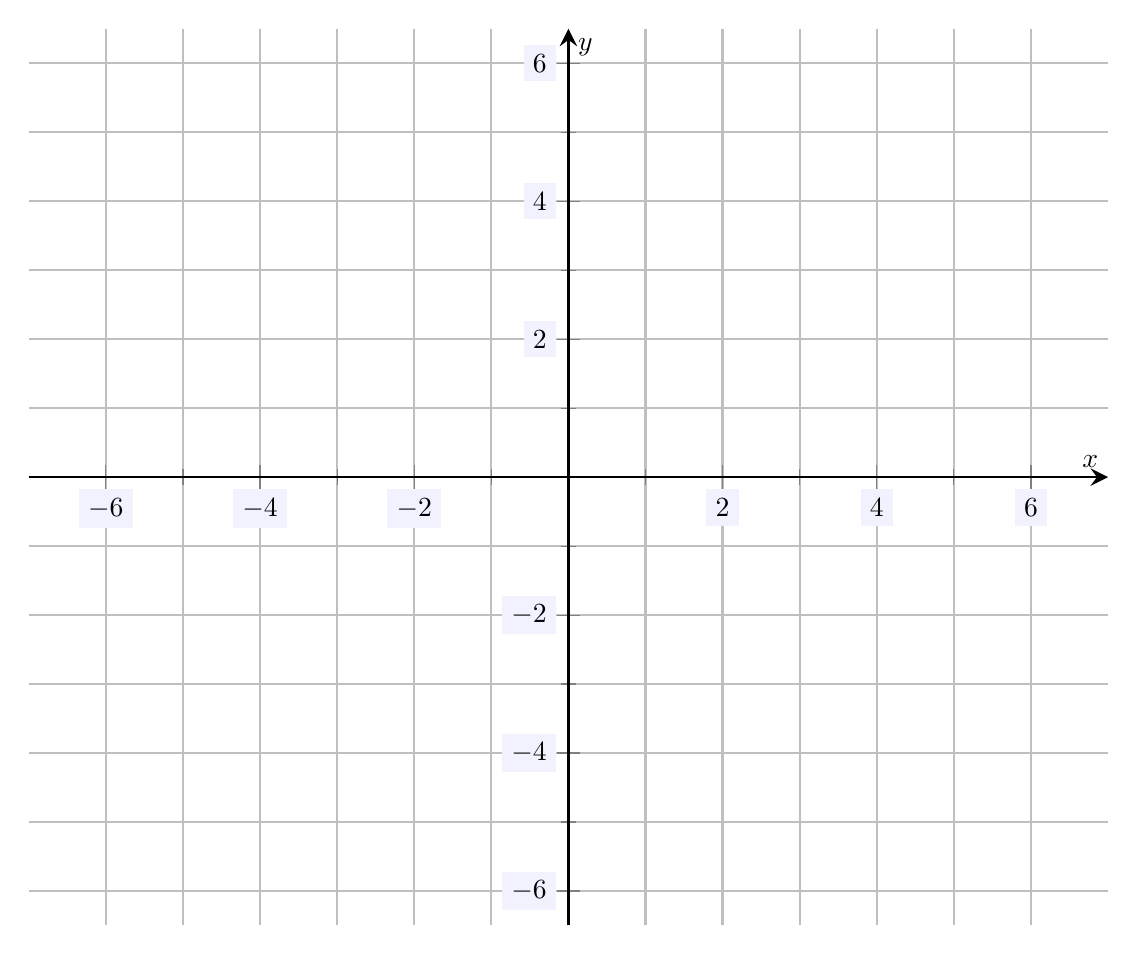
\begin{tikzpicture}[scale=2,every node/.style={scale=0.5}]
	\begin{axis}[
	grid=both,
	axis lines=middle,
	ticklabel style={fill=blue!5!white},
	xmin= -7, xmax=7,
	ymin= -6.5, ymax=6.5,
	xtick={-6,-4,-2,0,2,4,6},
	ytick={-6,-4,-2,0,2,4,6},
	minor tick = {-5,-3,...,5},
	xlabel=\(x\),ylabel=\(y\),
	]
	\end{axis}
	\end{tikzpicture}
	}
	\]





\newpage





% Problem 2
\problem{10} Plot the function $f(x):= x^2 + 4x - 1$, being as accurate as possible. 
	\[
	\fbox{
	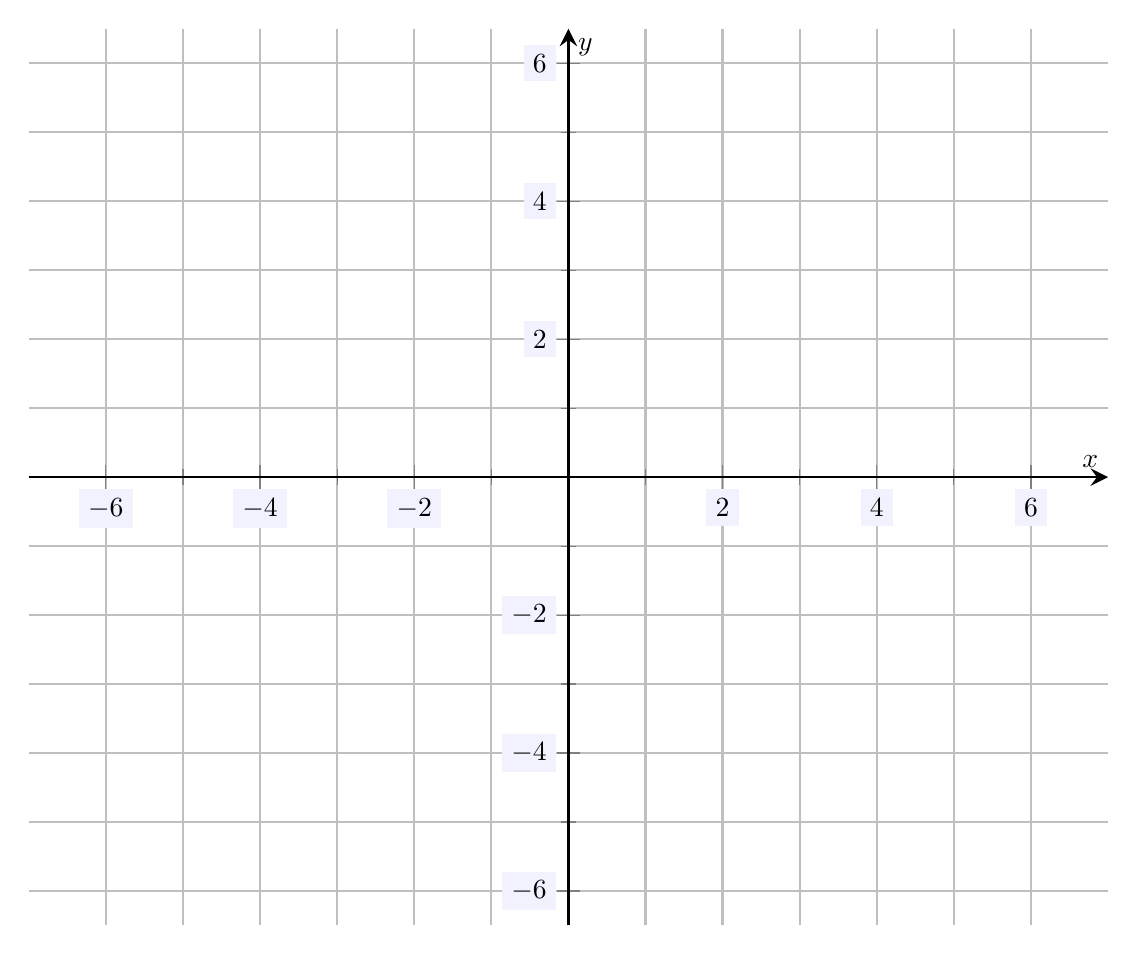
\begin{tikzpicture}[scale=2,every node/.style={scale=0.5}]
	\begin{axis}[
	grid=both,
	axis lines=middle,
	ticklabel style={fill=blue!5!white},
	xmin= -7, xmax=7,
	ymin= -6.5, ymax=6.5,
	xtick={-6,-4,-2,0,2,4,6},
	ytick={-6,-4,-2,0,2,4,6},
	minor tick = {-5,-3,...,5},
	xlabel=\(x\),ylabel=\(y\),
	]
	\end{axis}
	\end{tikzpicture}
	}
	\]





\newpage





% Problem 3
\problem{10} Plot the function $f(x):= \dfrac{x + 1}{x^2 + 1}$, being as accurate as possible. 
	\[
	\fbox{
	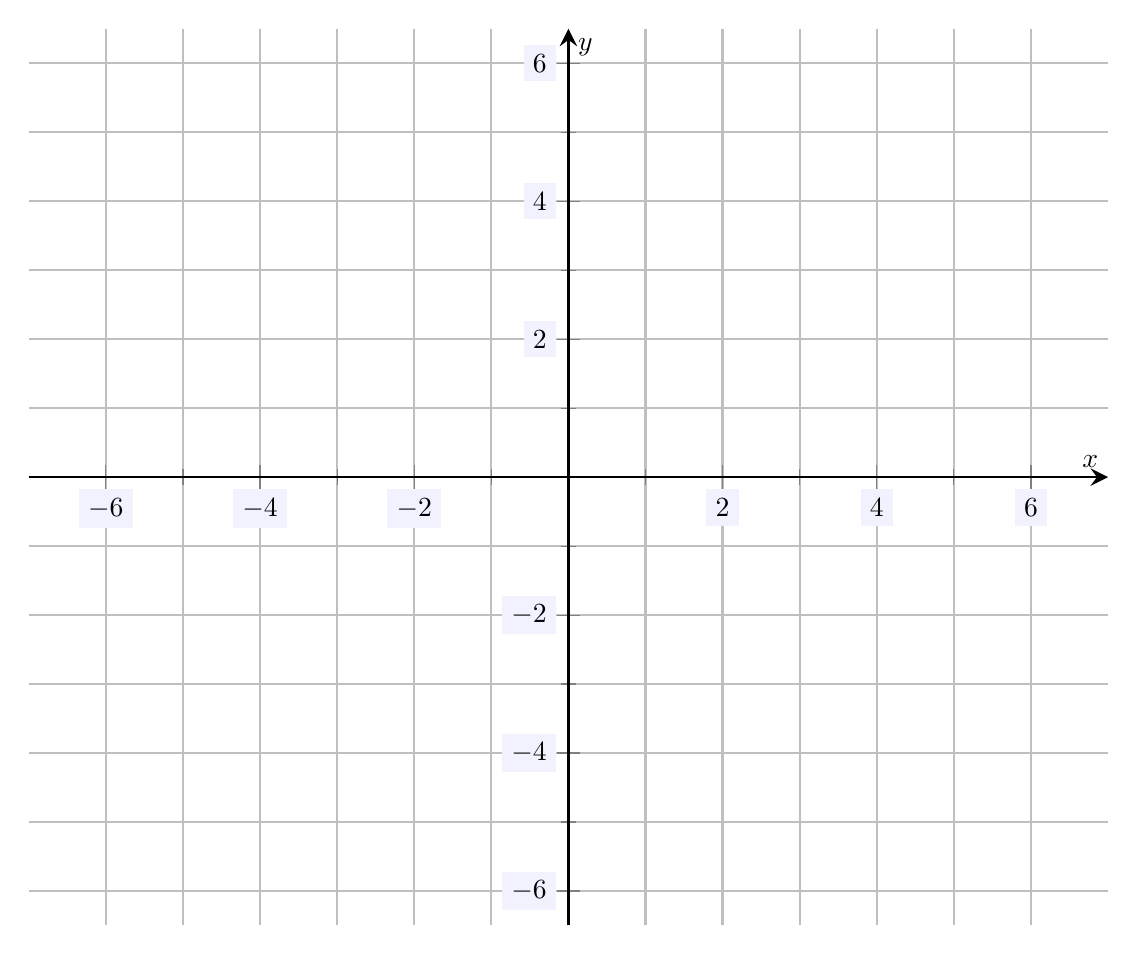
\begin{tikzpicture}[scale=2,every node/.style={scale=0.5}]
	\begin{axis}[
	grid=both,
	axis lines=middle,
	ticklabel style={fill=blue!5!white},
	xmin= -7, xmax=7,
	ymin= -6.5, ymax=6.5,
	xtick={-6,-4,-2,0,2,4,6},
	ytick={-6,-4,-2,0,2,4,6},
	minor tick = {-5,-3,...,5},
	xlabel=\(x\),ylabel=\(y\),
	]
	\end{axis}
	\end{tikzpicture}
	}
	\]





\newpage





% Problem 4
\problem{10} Let $f(x):= 5x - 3$.
	\begin{enumerate}[(a)]
	\item Find $f(1)$. \vfill
	\item What value(s) for $x$ make the output of $f(x)$ twice the output from (a)? \vfill
	\item Is $(1, 2)$ on the graph of $f(x)$? Explain. \vfill
	\item Is $(3, 5)$ on the graph of $f(x)$? Explain. \vfill
	\end{enumerate}





\newpage





% Problem 5
\problem{10} Define the following functions:
	\[
	\begin{aligned}
	f(x)&:= x^3 - x \\
	g(x)&:= x^2 - 2x + 3 \\
	h(x)&:= x^4 + x^2
	\end{aligned}
	\]
Determine if the functions $f(x)$, $g(x)$ and $h(x)$ are even functions, odd functions, or neither. Be sure to justify your answer. 





\newpage





% Problem 6
\problem{10} Consider the function $f(x)$ plotted below. 
	\[
	\fbox{
	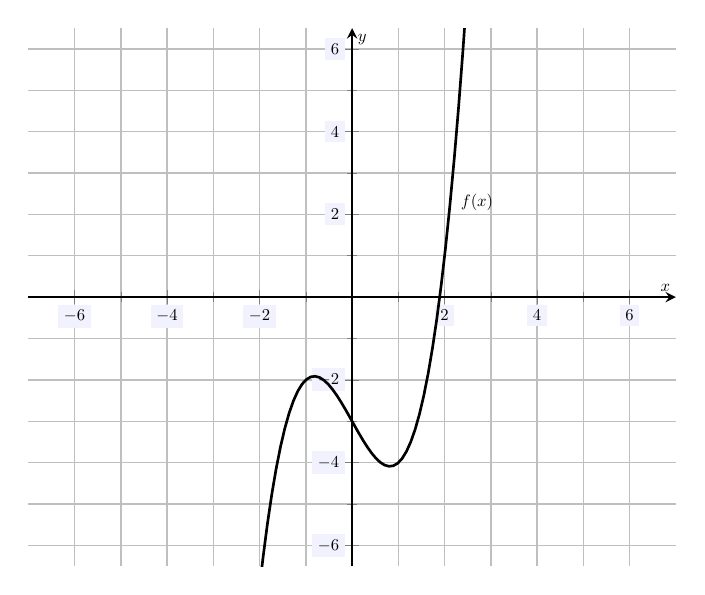
\begin{tikzpicture}[scale=1.2,every node/.style={scale=0.5}]
	\begin{axis}[
	grid=both,
	axis lines=middle,
	ticklabel style={fill=blue!5!white},
	xmin= -7, xmax=7,
	ymin= -6.5, ymax=6.5,
	xtick={-6,-4,-2,0,2,4,6},
	ytick={-6,-4,-2,0,2,4,6},
	minor tick = {-5,-3,...,5},
	xlabel=\(x\),ylabel=\(y\),
	samples=150
	]
	\node at (2.7,2.3) {$f(x)$};
	\addplot[thick,domain= -7:7] {x^3 - 2*x - 3};
	\end{axis}
	\end{tikzpicture}
	}
	\]

\begin{enumerate}[(a)]
\item What is $f(1)$? \vfill
\item Is the point $(2,1)$ on the graph of $f(x)$? Explain. \vfill
\item Is the point $(-2,-2)$ on the graph of $f(x)$? Explain. \vfill
\item Is the function $f(x)$ even, odd, or neither. Explain. \vfill
\end{enumerate}


%\printpoints
\end{document}